
\documentclass{article}
\usepackage{pgfplots}
\usepackage{pgfplotstable}
\usepackage{tikz}
\pgfplotsset{compat=1.8}
\begin{document}
    \begin{figure*}[t]
        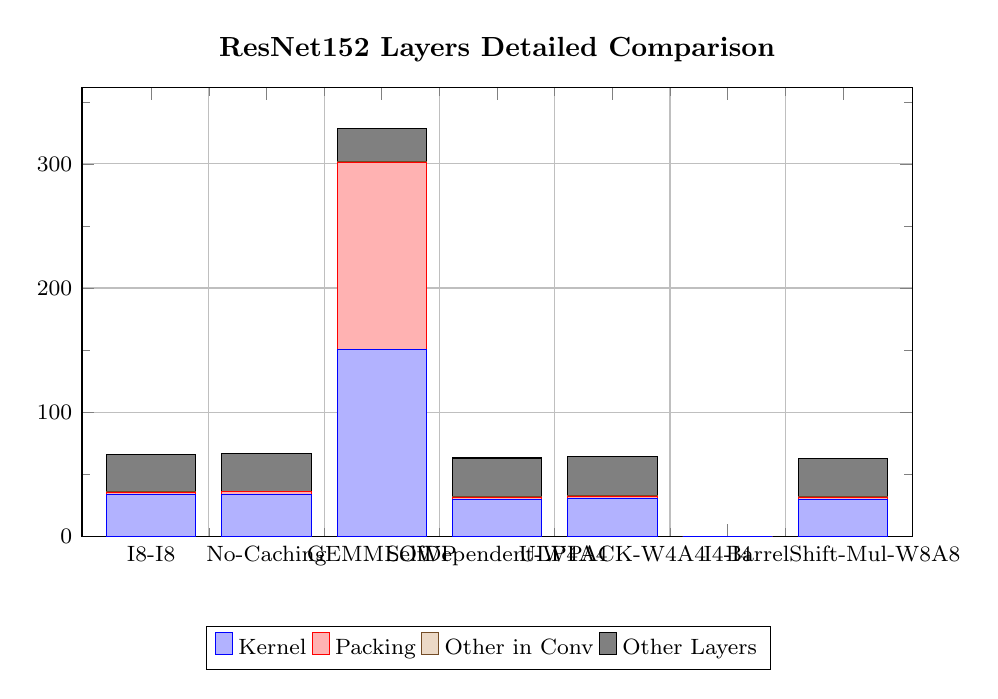
\begin{tikzpicture}
            \begin{axis}[
                ybar stacked,
                ymin=0.0,
                width=\linewidth,
                height=\axisdefaultheight,
                tick label style={font=\footnotesize},
                legend style={font=\tiny},
                label style={font=\footnotesize},
                symbolic x coords={I8-I8, No-Caching, GEMMLOWP, SelfDependent-W4A4, ULPPACK-W4A4, I4-I4, BarrelShift-Mul-W8A8},
                xtick=data,
                % ytick={0.60,0.80,1.0,1.2,1.4,1.6,1.8,2.0,2.2,2.4,2.6,2.8,3.0},
                align={center},
                bar width=7.5ex,
                legend columns=7,
                legend style={at={(0.49,-0.2)},anchor=north,font=\footnotesize},
                title=\textbf{ResNet152 Layers Detailed Comparison},
                ymajorgrids,
                xminorgrids = true,
                minor tick num=1
                ]
                \addplot coordinates { (I8-I8,33.33) (No-Caching,33.83) (GEMMLOWP,150.63) (SelfDependent-W4A4,29.66) (ULPPACK-W4A4,30.31) (I4-I4,0.00) (BarrelShift-Mul-W8A8,29.88) };
                \addplot coordinates { (I8-I8,1.85) (No-Caching,1.83) (GEMMLOWP,150.63) (SelfDependent-W4A4,1.64) (ULPPACK-W4A4,1.75) (I4-I4,0.00) (BarrelShift-Mul-W8A8,1.65) };
                \addplot coordinates { (I8-I8,0.45) (No-Caching,0.47) (GEMMLOWP,0.50) (SelfDependent-W4A4,0.55) (ULPPACK-W4A4,0.58) (I4-I4,0.00) (BarrelShift-Mul-W8A8,0.57) };
                \addplot coordinates { (I8-I8,29.88) (No-Caching,30.18) (GEMMLOWP,26.64) (SelfDependent-W4A4,31.16) (ULPPACK-W4A4,31.45) (I4-I4,0.00) (BarrelShift-Mul-W8A8,30.85) };
                \legend{
                    Kernel,
                    Packing,
                    Other in Conv,
                    Other Layers,
                };
            \end{axis}
        \end{tikzpicture}
    \end{figure*}
\end{document}
